%%
%% Copyright 2019-2024 Elsevier Ltd
%%
%% This file is part of the 'CAS Bundle'.
%% --------------------------------------
%%
%% It may be distributed under the conditions of the LaTeX Project Public
%% License, either version 1.3c of this license or (at your option) any
%% later version.  The latest version of this license is in
%%    http://www.latex-project.org/lppl.txt
%% and version 1.3c or later is part of all distributions of LaTeX
%% version 1999/12/01 or later.
%%
%% The list of all files belonging to the 'CAS Bundle' is
%% given in the file `manifest.txt'.
%%
%% Template article for cas-dc documentclass for
%% double column output.

\documentclass[a4paper,fleqn]{cas-dc}

% If the frontmatter runs over more than one page
% use the longmktitle option.

%\documentclass[a4paper,fleqn,longmktitle]{cas-dc}

\usepackage[numbers]{natbib}
%\usepackage[authoryear]{natbib}
% \usepackage[authoryear,longnamesfirst]{natbib}
\usepackage{microtype}
\usepackage{xurl}
\usepackage{siunitx}
\usepackage{tabularx}
\usepackage{tikz}
\usetikzlibrary{positioning, arrows.meta, automata}
\usepackage{amsthm}
\newtheorem{definition}{Definition}
\newtheorem{theorem}{Theorem}
\newtheorem{proposition}{Proposition}
%%%Author macros
\def\tsc#1{\csdef{#1}{\textsc{\lowercase{#1}}\xspace}}
\tsc{WGM}
\tsc{QE}
%%%

% Uncomment and use as if needed
%\newtheorem{theorem}{Theorem}
%\newtheorem{lemma}[theorem]{Lemma}
%\newdefinition{rmk}{Remark}
%\newproof{pf}{Proof}
%\newproof{pot}{Proof of Theorem \ref{thm}}

\begin{document}
\let\WriteBookmarks\relax
\def\floatpagepagefraction{1}
\def\textpagefraction{.001}

% Short title
\shorttitle{BASE: A Unified Biometric Driver Class for Embedded Real-Time Systems}

% Short author
\shortauthors{Md~Siratul~Islam and Md~Rasedujjaman}

% Main title of the paper
\title [mode = title]{BASE: A Unified Biometric Driver Class for Embedded Real-Time Systems}

% Title footnote mark
% eg: \tnotemark[1]
% \tnotemark[1]

% Title footnote 1.
% eg: \tnotetext[1]{Title footnote text}
% \tnotetext[1]{}

% First author
%
% Options: Use if required
% eg: \author[1,3]{Author Name}[type=editor,
%       style=chinese,
%       auid=000,
%       bioid=1,
%       prefix=Sir,
%       orcid=0000-0000-0000-0000,
%       facebook=<facebook id>,
%       twitter=<twitter id>,
%       linkedin=<linkedin id>,
%       gplus=<gplus id>]

\author[1,2]{Md~Siratul~Islam}[orcid=0009-0005-5945-8563]

% Footnote of the first author
% \fnmark[1]

% Email id of the first author
\ead{siratul.islam@linux.dev}

% URL of the first author
% \ead[url]{}

% Credit authorship
% eg: \credit{Conceptualization of this study, Methodology, Software}
\credit{Conceptualization, Methodology, Software, Investigation, Formal analysis, Writing -- original draft}

% Address/affiliation
\affiliation[1]{organization={Department of Physics, Shahjalal University of Science and Technology},
            city={Sylhet},
            citysep={}, % Uncomment if no comma needed between city and postcode
            postcode={3114},
            state={Sylhet},
            country={Bangladesh}}

\author[2]{Md~Rasedujjaman}[orcid=0000-0002-8276-1860]

% Corresponding author indication
\cormark[1]

% Footnote of the second author
% \fnmark[2]

% Email id of the second author
\ead{mrased-eee@sust.edu}

% URL of the second author
% \ead[url]{}

% Credit authorship
\credit{Supervision}

% Address/affiliation
\affiliation[2]{organization={Department of Electrical and Electronic Engineering, Shahjalal University of Science and Technology},
            city={Sylhet},
            citysep={}, % Uncomment if no comma needed between city and postcode
            postcode={3114},
            state={Sylhet},
            country={Bangladesh}}

% Corresponding author text
\cortext[1]{Corresponding author}

% Footnote text
% \fntext[1]{}

% For a title note without a number/mark
%\nonumnote{}

% Here goes the abstract
\begin{abstract}
Biometric modules speak vendor-specific protocols and enroll users in different ways, so embedded applications end up tied to one device family. We present the Biometric Abstraction for Secure Edge (BASE), a unified biometric driver class for resource-constrained real-time operating systems. BASE gives fingerprint, face, and palm modules one interface with capability discovery, typed results, and driver-enforced state, in synchronous and asynchronous modes. It supports both host-staged and device-managed enrollment, with defined cancellation and callback-lifetime rules. The core class is in Zephyr mainline. On an ESP32-S3 with two fingerprint modules and one face/palm module, one unchanged application source handled interrupted enrollment, re-enrollment, and identification on all three. All 54 accepted asynchronous operations delivered exactly one terminal event. Synchronous images added 4,972--5,328 bytes of linked ROM.
\end{abstract}

% Use if graphical abstract is present
%\begin{graphicalabstract}
%\includegraphics{}
%\end{graphicalabstract}

% Research highlights
\begin{highlights}
    \item BASE defines a unified biometric driver class for embedded real-time systems.
    \item The contract separates device persistence from host-side operation completion.
    \item One application handles enrollment, recovery, and matching across three families.
    \item Hardware tests characterize lifecycle behavior, scheduling, and memory costs.
    \item The core biometrics driver class is integrated into Zephyr mainline.
\end{highlights}

%\nocite{*}

% Keywords
% Each keyword is seperated by \sep
\begin{keywords}
    Embedded Systems \sep Hardware Abstraction \sep Real-Time Operating Systems \sep Device Drivers \sep Zephyr RTOS
\end{keywords}

\maketitle

% Main text
\section{Introduction}
\label{sec:introduction}

Biometric modules differ not only in protocol but in who controls enrollment and when a template is stored, so an application written for one module rarely works with another. A common biometric driver class can encapsulate these differences while applications share enrollment, matching, and template-management logic. In a resource-constrained real-time operating system (RTOS), this interface must also coexist with sensing, communication, and control. This systems problem complements research on recognition, template protection, and authentication security~\cite{yang2021biometric,ahvanooey2022modern}.

BioAPI and Embedded BioAPI define common biometric interfaces~\cite{iso19784,iso29164}, while libfprint and fprintd provide a fingerprint-device interface in Linux userspace~\cite{libfprint_device_api,fprintd_device_api}. Zephyr's \texttt{grow\_r502a} instead exposes biometric operations through sensor attributes and \texttt{sensor\_value} fields~\cite{zephyr_sensor_api,zephyr_r502a}. BASE targets a dedicated RTOS driver class with shared enrollment, matching, and termination semantics across host-staged and device-managed modules.

Some modules require host-controlled capture stages; others manage acquisition and storage internally. Even staged devices may store templates during the final capture or a later finalization command, so a common call sequence cannot imply a common persistence boundary.

Split-phase interfaces separate initiation from completion~\cite{gay2003nesc}, while cancellation can introduce concurrency errors~\cite{sethi2022cancellation}. Biometric interfaces must distinguish outcomes, terminal notification, and device release: enrollment may succeed before cleanup, and cancellation need not reverse storage. These boundaries determine callback lifetime and safe device reuse.

We present the \emph{Biometric Abstraction for Secure Edge} (BASE), a unified biometric driver class whose core is integrated into Zephyr mainline~\cite{zephyr_biometrics}; the evaluated multimodal and asynchronous extensions are under upstream review~\cite{zephyr_pr2}. BASE combines capability discovery, typed operations and results, and explicit lifecycle rules. Applications select supported workflows; drivers translate protocols and enforce state. The architecture separates application policy, the subsystem contract, and device-specific execution. Portability concerns shared workflows and operation semantics; biometric fusion, template-format interoperability, and score calibration remain outside its scope.

We investigate four research questions. \textbf{RQ1:} How can a common RTOS biometric contract accommodate differences in capabilities, enrollment ownership, and storage? \textbf{RQ2:} Does the asynchronous implementation satisfy termination, conflicting-operation exclusion, and callback-quiescence obligations in directed tests? \textbf{RQ3:} How do driver implementation, operating mode, priority, and background load affect a concurrent periodic task's response times? \textbf{RQ4:} What linked ROM and RAM costs and observed stack usage do the implementations incur?

The contributions are:
\begin{itemize}
    \item \textbf{A unified RTOS biometric driver class} combining capability-dependent workflows, typed results, and driver-enforced state.
    \item \textbf{Explicit lifecycle semantics} for enrollment, persistence, cancellation, and callback lifetime, including cancellation that does not assume rollback of a stored template.
    \item \textbf{Three heterogeneous device mappings.} ZFM-X0 and GT-5X fingerprint drivers and an AI10 face/palm driver preserve distinct enrollment, storage, and recovery behavior.
    \item \textbf{An ESP32-S3 evaluation} of application reuse, functional coverage, lifecycle behavior, scheduling interference, linked memory, source-derived heap allocation requests, and observed stack usage.
\end{itemize}

The architecture and driver mappings address RQ1, supported by E1; E2--E4 address RQ2--RQ4. Section~\ref{sec:related_work} reviews related work; Sections~\ref{sec:architecture} and~\ref{sec:implementation} describe BASE; Section~\ref{sec:evaluation} evaluates it; and Section~\ref{sec:conclusion} concludes.
\section{Related Work and Motivation}
\label{sec:related_work}

Biometric surveys examine recognition, template protection, and authentication security \cite{yang2021biometric,ahvanooey2022modern}. Here, we compare the host interfaces used to integrate biometric modules into an RTOS running on a microcontroller (MCU), focusing on capabilities, enrollment, outcomes, and operation lifetime.

\subsection{Biometric Standards and Integration Frameworks}

BioAPI defines cross-vendor application and service-provider interfaces \cite{iso19784}; Gonz\'{a}lez-Agulla et al. provide a Java Native Interface wrapper for Windows and Linux/Unix \cite{gonzalezagulla2009bioapi}. Embedded BioAPI specifies commands for constrained biometric modules while leaving low-level implementation outside its scope \cite{iso29164}. BASE maps heterogeneous module protocols into an RTOS driver contract without claiming conformance to either standard.

Milovanovi\'{c} et al. demonstrate multimodal integration through adapters, capability discovery, component-state tracking, and sessions \cite{milovanovic2012interoperability}. Their Java framework integrates face, fingerprint, and voice, establishing precedents for capability-aware integration.

\subsection{Linux and Android Biometric Interfaces}

The fprint project separates device support in \texttt{libfprint} from application access through the \texttt{fprintd} D-Bus service~\cite{libfprint_device_api,fprintd_device_api}. The current libfprint \texttt{FpDevice} interface provides feature discovery, enrollment progress, device-storage operations, and synchronous and asynchronous execution \cite{libfprint_device_api}. Its matching callback can report an outcome before operation completion, and a subsequent failure can be reported at completion. Its asynchronous enrollment interface initiates one operation with progress and completion callbacks, accepting a \texttt{GCancellable} for cancellation. BASE adopts the established distinction between outcome and completion while exposing application-issued capture/finalize steps alongside device-managed enrollment. Its stop operation is device-scoped, so applications must coordinate ownership rather than associate cancellation with a request object.

The fprintd service provides device claiming and requires \texttt{EnrollStop} after successful enrollment status, separating outcome delivery from completion~\cite{fprintd_device_api}. Android's \texttt{BiometricPrompt} provides system-mediated authentication with capability checks and outcome callbacks~\cite{android_bio}. BASE exposes RTOS module operations, including application-controlled enrollment where supported.

\subsection{Biometric Integration in MCU RTOSs}

\subsubsection{Module-Specific Packages and Vendor Frameworks}

RT-Thread's \texttt{as608} package supports AS60x fingerprint modules through image acquisition, feature generation, template construction and storage, search, and enrollment helpers \cite{rtthread_as608}. It provides a module-family interface rather than a driver class shared across protocols and modalities.

NXP's EdgeReady i.MX RT117F solution runs a face-recognition stack on FreeRTOS, with camera and algorithm managers, hardware abstraction layers, and a facial biometric API and runtime \cite{nxp_rt117f_face}. Its MCU executes vision processing, whereas BASE controls modules that perform acquisition and recognition internally.

\subsubsection{Zephyr's Generic Sensor Interface}
\label{sec:sensor_limitations}

Zephyr's sensor subsystem provides channels, attributes, triggers, and blocking and non-blocking acquisition \cite{zephyr_sensor_api}. Its \texttt{grow\_r502a} driver and sample expose record addition, lookup, deletion, and free-index selection through sensor attributes, with a touch trigger for enrollment and matching results containing an identifier and confidence \cite{zephyr_r502a,zephyr_r502a_sample}.

This provides working biometric integration, but applications depend on the driver-specific public definitions in \texttt{grow\_r502a.h} and must interpret the biometric meanings assigned to its sensor attributes and values \cite{zephyr_r502a}. A dedicated biometric contract makes enrollment progress, template identifiers, modalities, and outcomes explicit across drivers. It must also describe who controls acquisition and how host-visible progress relates to device storage, since shared acquisition mechanisms alone do not define those semantics.

\subsection{Operation Lifetime and RTOS Concurrency}

The nesC/TinyOS model separates initiation from completion through split-phase commands and events \cite{gay2003nesc}; biometric frameworks likewise provide asynchronous operations. Sethi et al. document cancellation requirements and failures in concurrent and distributed systems \cite{sethi2022cancellation}. For enrollment, cancellation must account for stored templates, outcomes already delivered, outstanding callbacks, and subsequent device access.

Execution mode alone also does not determine scheduling interference: synchronous calls may suspend their callers, while asynchronous workers consume CPU time when runnable. Zephyr's scheduling and synchronization mechanisms govern their interaction with other tasks \cite{zephyr_docs}, motivating measurements under stated priorities and workloads.

\subsection{Architectural Positioning and Requirements}

Table~\ref{tab:gap_matrix} positions BASE as a unified RTOS biometric driver class. Capability discovery, typed interfaces, and asynchronous completion have established precedents. BASE integrates these mechanisms across heterogeneous enrollment and storage behaviors: capabilities select workflows, drivers enforce state, typed results support shared application logic, and lifecycle rules govern cancellation and reuse. The contribution comprises this integrated contract, three device-family mappings, and an evaluated Zephyr implementation.

\begin{table*}[!t]
\centering
\caption{Architectural comparison of the reviewed biometric interfaces and implementations.}
\label{tab:gap_matrix}
\small
\renewcommand{\arraystretch}{1.18}
\setlength{\tabcolsep}{4pt}
\begin{tabularx}{\textwidth}{|>{\raggedright\arraybackslash}p{0.16\textwidth}|*{3}{>{\raggedright\arraybackslash}X|}}
\hline
\textbf{Approach} &
\textbf{Interface and device scope} &
\textbf{Workflow and lifecycle abstraction} &
\textbf{Implementation setting} \\
\hline
BioAPI \cite{iso19784} &
Standard application and service-provider interfaces across vendors &
Common service operations; framework-based or framework-free integration &
Platform-specific implementation of a standard \\
\hline
Embedded BioAPI \cite{iso29164} &
Command interface for constrained biometric modules &
Commands implemented by conforming modules &
Embedded systems; low-level implementation outside scope \\
\hline
Multimodal framework \cite{milovanovic2012interoperability} &
Adapters for biometric software, devices, and databases &
Functionality discovery, component states, and sessions &
Java implementation: face, fingerprint, and voice \\
\hline
libfprint / fprintd \cite{libfprint_device_api,fprintd_device_api} &
Fingerprint device library and D-Bus service &
Enrollment progress, separate matching outcome and completion, cancellation; service-level device claiming &
Linux userspace library and service \\
\hline
Android biometrics \cite{android_bio} &
Application authentication framework &
Capability checks, system-mediated authentication, and outcome callbacks &
Android platform services \\
\hline
RT-Thread \texttt{as608} \cite{rtthread_as608} &
AS60x fingerprint module-family interface &
Capture, template construction and storage, search, and enrollment helpers &
RT-Thread peripheral package \\
\hline
NXP EdgeReady i.MX RT117F \cite{nxp_rt117f_face} &
Vendor facial biometric API and runtime &
Camera/algorithm managers and hardware abstraction; cancellation not detailed in cited fact sheet &
MCU vision-processing stack on FreeRTOS \\
\hline
Zephyr \texttt{grow\_\allowbreak{}r502a} \cite{zephyr_r502a_sample} &
Fingerprint operations through the sensor interface &
Record attributes, matching results, and touch trigger &
Device-specific RTOS sensor driver and sample \\
\hline
\textbf{BASE} &
Biometric driver contract; fingerprint, face, and palm drivers &
Capability-aware staged/device-managed enrollment; terminal-event and callback-quiescence obligations &
Zephyr driver class; driver-specific state and execution \\
\hline
\end{tabularx}

\par\smallskip
\begin{minipage}{\textwidth}
\footnotesize
\textit{Scope:} Entries summarize the cited interfaces; undocumented properties are left unspecified.
\end{minipage}
\end{table*}

The comparison motivates five requirements:
\begin{enumerate}
\item \textbf{Explicit biometric semantics:} shared capabilities, identifiers, enrollment progress, modalities, and outcomes.
\item \textbf{Capability-aware portability:} workflow discovery and defined errors for absent operations or unsupported parameters.
\item \textbf{Heterogeneous enrollment ownership:} staged and device-managed acquisition, with progress distinguished from storage.
\item \textbf{Defined operation lifetimes:} acceptance, outcomes, termination, callback context and quiescence, cancellation, and conflicting access.
\item \textbf{Accountable RTOS resource use:} execution behavior, scheduling effects, memory costs, and observed stack usage under stated configurations.
\end{enumerate}

Requirements~1--3 address RQ1, Requirement~4 addresses RQ2, and Requirement~5 addresses RQ3--RQ4. Section~\ref{sec:architecture} develops the contract and assigns responsibilities.
\section{The BASE Architecture}
\label{sec:architecture}

BASE defines common biometric operations while preserving differences in acquisition ownership, storage, and execution. Applications select capability-dependent workflows; drivers translate requests and enforce the shared behavioral contract.

\subsection{Three-Plane Architecture and Responsibilities}

Figure~\ref{fig:architecture} separates three responsibilities. The \textbf{application plane} selects workflows, coordinates device ownership, and applies policy. Template identifiers refer to device-local records; associating them with users or authorization decisions remains an application task.

The \textbf{subsystem contract plane} defines operations, typed results, optional-handler checks, and lifecycle obligations. Zephyr's \texttt{biometric\_\allowbreak{}driver\_\allowbreak{}api} binds handlers to device instances for inline dispatch.

The \textbf{driver implementation plane} translates commands and responses and coordinates protocol and device state. Enforcement resides here because acquisition recovery, storage transitions, and cleanup depend on device protocols. Drivers can use different execution mechanisms while satisfying the same externally observable obligations.

This flexibility requires repeated admission and completion bookkeeping and validation of each driver's conformance. Shared helpers could centralize that bookkeeping while retaining protocol-specific transitions. BASE currently uses driver-local enforcement; the evaluation characterizes its costs without comparing it with centralized enforcement.

\begin{figure}
\centering
\definecolor{baseGray}{HTML}{666666}
\definecolor{baseBlue}{HTML}{0072B2}
\definecolor{baseOrange}{HTML}{D55E00}
\begin{tikzpicture}[
    x=\columnwidth,y=1cm,
    font=\sffamily\footnotesize,
    box/.style={draw=baseGray,rounded corners=1.5pt,align=center,line width=0.6pt,inner sep=3pt},
    call/.style={-{Stealth[length=1.5mm]},draw=black!75,line width=0.65pt,shorten <=1pt,shorten >=1pt},
    reply/.style={call,dashed},
    lab/.style={font=\sffamily\footnotesize,fill=white,inner sep=1.5pt}
]
\node[box,fill=baseGray!7,text width=0.90\columnwidth,minimum height=1.05cm] (app) at (0,0) {\textbf{Application plane}\\Discover capabilities; select workflows;\\apply policy; consume outcomes};
\node[box,draw=baseBlue,fill=baseBlue!8,text width=0.90\columnwidth,minimum height=1.20cm] (contract) at (0,-1.85) {\textbf{Subsystem contract plane}\\Types, operations, and API dispatch;\\optional-operation checks; lifecycle obligations};
\draw[call] ([xshift=-0.22\columnwidth]app.south) -- node[lab,left=1pt]{requests} ([xshift=-0.22\columnwidth]contract.north);
\draw[reply] ([xshift=0.22\columnwidth]contract.north) -- node[lab,right=1pt]{results/events} ([xshift=0.22\columnwidth]app.south);
\draw[draw=baseOrange,fill=baseOrange!3,rounded corners=2pt,line width=0.6pt] (-0.49,-3.02) rectangle (0.49,-5.55);
\node[box,draw=baseOrange,fill=baseOrange!8,text width=0.265\columnwidth,minimum height=1.60cm] (zfm) at (-0.325,-3.95) {\textbf{ZFM-X0}\\Fingerprint\\Staged enrollment\\Protocol/state};
\node[box,draw=baseOrange,fill=baseOrange!8,text width=0.265\columnwidth,minimum height=1.60cm] (gt) at (0,-3.95) {\textbf{GT-5X}\\Fingerprint\\Staged enrollment\\Protocol/state};
\node[box,draw=baseOrange,fill=baseOrange!8,text width=0.265\columnwidth,minimum height=1.60cm] (ai) at (0.325,-3.95) {\textbf{AI10}\\Face/palm\\Device-managed\\Worker/events};
\foreach \drv in {zfm,gt,ai}{
    \coordinate (request) at ([xshift=-2mm]\drv.north);
    \coordinate (result) at ([xshift=2mm]\drv.north);
    \draw[call] (contract.south -| request) -- (request);
    \draw[reply] (result) -- (contract.south -| result);
}
\node[align=center,text=baseOrange!80!black,text width=0.90\columnwidth] at (0,-5.17) {\textbf{Driver implementation plane}\\Device-specific protocols and state enforcement};
\end{tikzpicture}
\caption{Three-plane architecture of BASE. Solid arrows denote requests; dashed arrows denote results or events. Each driver implements the shared contract for its module; protocol and state enforcement remain driver-local.}
\label{fig:architecture}
\end{figure}

\subsection{Capabilities, Operations, and Outcomes}

Applications query capabilities to select supported workflows. Capabilities report modalities, storage modes, template capacity and size, staged sample count, and asynchronous operation categories. A positive sample count selects staged enrollment; zero denotes device-managed enrollment, for which asynchronous enrollment support must also be advertised.

Discovery does not enumerate every attribute, matching mode, timeout range, or identifier-allocation policy. Applications therefore combine capability checks with operation errors: an absent optional handler returns \texttt{-ENOSYS}, whereas an implemented operation can reject unsupported parameters with \texttt{-ENOTSUP} or invalid arguments with \texttt{-EINVAL}.

Capability queries, synchronous matching, and individual template deletion are mandatory handlers. Staged enrollment, inventory and transfer operations, bulk deletion, attributes, LED control, and asynchronous operations are optional. Advertising asynchronous operations additionally requires callback registration and stop support. Device storage does not itself imply template import/export support.

Verification compares against a specified template; identification searches the database. These meanings are independent of execution mode: synchronous calls return outcomes directly, while asynchronous requests deliver events. For example, AI10 supports synchronous and asynchronous identification but rejects verification.

Typed results separate matching identifiers and scores, capture progress, and enrollment outcomes. Asynchronous events carry discriminated payloads. Supported modalities describe the device; each successful result identifies its own modality. AI10 advertises face and palm and selects modality automatically during asynchronous matching.

Confidence remains device-specific; match image quality uses a 0--100 representation. Zero can indicate unavailable confidence or quality, and neither field establishes cross-device calibration. Associating templates with people, combining scores, and transferring templates between incompatible formats remain outside the contract.

\subsection{Enrollment Models and State Transitions}

BASE exposes staged and device-managed enrollment because they assign acquisition control differently. A single whole-enrollment operation could accommodate both internally, but would remove application control over individual capture steps from the common interface. Conversely, requiring capture steps for autonomous modules would expose transitions the host cannot command. BASE therefore retains both workflows and selects between them through capabilities.

Portability concerns operation meanings and workflow selection rather than identical recovery actions. Applications retain responsibility for identifier allocation, session ownership, and reconciliation after uncertain storage outcomes. Inventory operations support reconciliation where available; otherwise, the common contract cannot establish whether an interrupted exchange changed device storage. Cancellation and host-state reset consequently provide no general rollback guarantee.

\subsubsection{Host-Controlled Staged Enrollment}

A session begins with \texttt{biometric\_\allowbreak{}enroll\_\allowbreak{}start()}. The application collects samples through repeated calls to \texttt{biometric\_\allowbreak{}enroll\_\allowbreak{}capture()}, then calls \texttt{biometric\_\allowbreak{}enroll\_\allowbreak{}finalize()} to complete enrollment. Applications follow reported progress: ZFM-X0 requires two captures and GT-5X three. Figure~\ref{fig:fsm}(a) shows successful progression. Let $I$ denote idle and $C_k$ a session with $k$ accepted captures for a device requiring $N$ samples:
\begin{align}
\delta(I,\mathrm{start}_{\mathrm{ok}})&=C_0, \\
\delta(C_k,\mathrm{capture}_{\mathrm{ok}})&=C_{k+1},\quad 0\leq k<N, \\
\delta(C_N,\mathrm{finalize}_{\mathrm{ok}})&=I.
\end{align}
State $C_N$ denotes readiness for finalization. Capture is rejected in idle or ready states, and finalization before readiness. Abort resets host state where implemented.

Recovery differs by driver. ZFM-X0 resets progress after acquisition or feature-conversion failure; argument and sequencing checks may reject a call without running that sequence. GT-5X preserves its stage after acquisition or enrollment-command failure. Where abort is supported, applications can abort and restart, handling an already-idle response.

ZFM-X0 creates and stores the template during finalization. GT-5X stores during its third capture; finalization closes host state and attempts to refresh the enrollment count without issuing a storage command. Readiness therefore describes workflow progress, and abort cannot be assumed to undo storage (Section~\ref{sec:implementation}).

\begin{figure*}[!t]
\centering
\definecolor{baseGray}{HTML}{666666}
\definecolor{baseBlue}{HTML}{0072B2}
\definecolor{baseOrange}{HTML}{D55E00}
\resizebox{\textwidth}{!}{%
\begin{tikzpicture}[
    x=1cm,y=1cm,font=\sffamily\small,
    state/.style={draw=baseGray,rounded corners=2pt,align=center,line width=0.7pt,text width=3.15cm,minimum height=0.64cm,inner sep=4pt,fill=baseGray!7},
    staged/.style={draw=baseBlue,fill=baseBlue!8},
    managed/.style={draw=baseOrange,fill=baseOrange!8},
    arrow/.style={-{Stealth[length=1.8mm]},line width=0.75pt,shorten <=1pt,shorten >=1pt},
    stagedarrow/.style={arrow,draw=baseBlue},
    managedarrow/.style={arrow,draw=baseOrange},
    lab/.style={font=\sffamily\footnotesize,align=center,fill=white,inner sep=2pt}
]
\node[font=\sffamily\bfseries,text=baseBlue!85!black] at (3.8,0.15) {(a) Host-controlled staged enrollment};
\node[font=\sffamily\bfseries,text=baseOrange!80!black] at (12.0,0.15) {(b) Device-managed enrollment};
\draw[baseGray!30] (8,-0.35) -- (8,-6.42);
\node[state] (si) at (3.1,-0.70) {Idle};
\node[state,staged] (sc) at (3.1,-2.20) {Capturing\\$0\leq k<N$};
\node[state,staged] (sr) at (3.1,-4.00) {Ready\\$k=N$};
\draw[stagedarrow] (si.south) -- node[lab,right=3pt]{start succeeds} (sc.north);
\draw[stagedarrow] (sc.south) -- node[lab,right=3pt]{final capture\\succeeds} (sr.north);
\draw[stagedarrow] ([yshift=-1.5mm]sc.east) -- (6.8,-2.35) -- (6.8,-2.05) -- ([yshift=1.5mm]sc.east);
\node[lab,text width=2.2cm] at (6.40,-2.88) {capture succeeds;\\$k\gets k+1$ ($<N$)};
\draw[stagedarrow] (sr.west) -- (0.90,-4.00) -- (0.90,-0.70) -- (si.west);
\node[lab,rotate=90] at (0.48,-2.50) {finalize succeeds};
\node[align=left,text width=6.9cm,font=\sffamily\footnotesize] at (3.8,-5.72) {Successful progress is shown. Abort resets host state; capture failures may preserve or discard progress depending on the driver. Ready is a logical state, not a universal storage boundary.};
\node[state] (ai) at (11.1,-0.70) {Idle};
\node[state,managed] (aa) at (11.1,-2.20) {Active\\Device owns capture};
\node[state,managed] (ac) at (11.1,-3.73) {Protocol cleanup};
\node[state,managed] (as) at (11.1,-5.08) {Terminal callback\\\texttt{STOPPED}; still busy};
\draw[managedarrow] (ai.south) -- node[lab,right=3pt]{request\\accepted} (aa.north);
\draw[managedarrow] (aa.south) -- node[lab,right=3pt]{completion, failure,\\or cancellation} (ac.north);
\draw[managedarrow] (ac.south) -- node[lab,right=3pt]{\texttt{ERROR} if needed} (as.north);
\draw[managedarrow] (as.west) -- (8.95,-5.08) -- (8.95,-0.70) -- (ai.west);
\node[lab,rotate=90] at (8.52,-3.18) {callback returns; release activity};
\node[lab,align=left,text width=2.35cm] at (14.72,-1.78) {Success emits\\\texttt{ENROLL\_\allowbreak{}}\texttt{COMPLETE}\\with ID and modality\\before cleanup.};
\node[align=left,text width=6.9cm,font=\sffamily\footnotesize] at (12,-6.17) {A stored template can survive cancellation or cleanup failure. The device is available only after the terminal callback returns.};
\end{tikzpicture}%
}
\caption{Enrollment models. Panel (a) abstracts successful staged progress, with driver-specific error recovery. Panel (b) shows the host lifecycle for device-managed enrollment; the module owns acquisition and storage. Neither panel treats cancellation as rollback.}
\label{fig:fsm}
\end{figure*}

\subsubsection{Device-Managed Enrollment}

\texttt{biometric\_\allowbreak{}enroll\_\allowbreak{}async()} delegates capture and storage to the module. A successful call confirms acceptance; \texttt{ENROLL\_\allowbreak{}COMPLETE} subsequently reports a successful enrollment's stored identifier and modality. Cleanup and terminal delivery conclude the host operation (Figure~\ref{fig:fsm}(b)); the internal capture count need not be exposed.

The interface accepts an identifier or \texttt{BIOMETRIC\_\allowbreak{}ID\_\allowbreak{}AUTO} for device allocation. AI10 supports automatic allocation only, advertises zero staged samples and asynchronous enrollment, and supplies no staged handlers. Stopping controls execution subject to the persistence semantics in Section~\ref{sec:correctness_properties}.

\subsection{Asynchronous Lifecycle and Concurrency}
\label{sec:interrupt_io}

\subsubsection{Acceptance, Results, and Termination}

Request acceptance, biometric outcomes, terminal notification, and release of device activity are separate boundaries (Figure~\ref{fig:async_lifecycle}). Callback registration occurs while idle and persists across operations. Callback-visible state must be initialized before submission because callbacks may begin before the initiating call returns.

Matching emits \texttt{MATCH} or \texttt{NO\_\allowbreak{}MATCH} per attempt; successful enrollment emits \texttt{ENROLL\_\allowbreak{}COMPLETE}. An unsuccessful attempt need not end continuous recognition. Operation or cleanup failures produce \texttt{ERROR}; \texttt{STOPPED} terminates the lifecycle. Effective cancellation may emit \texttt{STOPPED} with \texttt{-ECANCELED} without an additional error event.

Outcome and lifecycle status differ: \texttt{NO\_\allowbreak{}MATCH} can precede \texttt{STOPPED}(0) after normal completion, while successful enrollment can precede cleanup failure, \texttt{ERROR}, and a failing \texttt{STOPPED}. Table~\ref{tab:lifecycle_contract} assigns driver and application obligations.

\begin{figure*}[t]
\centering
\definecolor{baseGray}{HTML}{666666}
\definecolor{baseBlue}{HTML}{0072B2}
\definecolor{baseOrange}{HTML}{D55E00}
\resizebox{\textwidth}{!}{%
\begin{tikzpicture}[
    x=1cm,y=1cm,font=\sffamily\footnotesize,
    arrow/.style={-{Stealth[length=1.6mm]},draw=baseGray!85!black,line width=0.65pt},
    ret/.style={arrow,dashed},
    completion/.style={draw=baseBlue},
    cancellation/.style={draw=baseOrange},
    msg/.style={midway,above,fill=white,inner sep=1pt,align=center},
    head/.style={draw=baseGray,fill=baseGray!7,rounded corners=1pt,line width=0.6pt,text width=3.5cm,align=center,minimum height=0.55cm}
]
\node[head] (app) at (2.2,0) {\textbf{Application interface}};
\node[head,draw=baseOrange,fill=baseOrange!8] (worker) at (8,0) {\textbf{Biometric driver}};
\node[head,draw=baseOrange!75!black,fill=baseOrange!3] (module) at (13.8,0) {\textbf{Biometric module}};
\coordinate (lifeline end) at (0,-8.20);
\foreach \actor in {app,worker,module}{
    \draw[densely dashed,baseGray!50] (\actor.south) -- (lifeline end -| \actor.south);
}
\draw[arrow] (2.2,-0.85) -- node[msg]{\texttt{match\_async} / \texttt{enroll\_async}} (8,-0.85);
\draw[ret] (8,-1.28) -- node[msg]{return 0: accepted, not completed} (2.2,-1.28);
\draw[arrow] (8,-1.71) -- node[msg]{protocol setup and operation command} (13.8,-1.71);
\draw[baseGray!75,line width=0.6pt] (0.16,-1.98) rectangle (15.84,-8.30);
\node[anchor=north west,fill=baseBlue!8,text=baseBlue!85!black,inner sep=3pt] at (0.16,-1.98) {\textbf{Completion path} (one successful attempt)};
\draw[ret,completion] (13.8,-2.75) -- node[msg]{successful result} (8,-2.75);
\draw[arrow,completion] (8,-3.20) -- node[msg]{\texttt{MATCH} or \texttt{ENROLL\_COMPLETE}} (2.2,-3.20);
\draw[arrow,completion] (8,-3.65) -- node[msg]{protocol cleanup} (13.8,-3.65);
\draw[ret,completion] (13.8,-4.10) -- node[msg]{cleanup acknowledgment} (8,-4.10);
\draw[arrow,completion] (8,-4.55) -- node[msg]{\texttt{STOPPED}(0); device still busy} (2.2,-4.55);
\node[anchor=west,fill=white,text=baseBlue!85!black,inner sep=1.5pt] at (8.16,-4.88) {Callback returns; mark idle.};
\draw[dashed,baseGray!75] (0.16,-5.18) -- (15.84,-5.18);
\node[anchor=north west,fill=baseOrange!8,text=baseOrange!80!black,inner sep=3pt] at (0.16,-5.18) {\textbf{Cancellation path} (cancellation takes effect)};
\draw[arrow,cancellation] (2.2,-5.95) -- node[msg]{\texttt{async\_stop}; caller waits} (8,-5.95);
\draw[arrow,cancellation] (8,-6.40) -- node[msg]{interrupt wait; protocol cleanup} (13.8,-6.40);
\draw[ret,cancellation] (13.8,-6.85) -- node[msg]{cleanup acknowledgment} (8,-6.85);
\draw[arrow,cancellation] (8,-7.30) -- node[msg]{\texttt{STOPPED}(-\texttt{ECANCELED}); still busy} (2.2,-7.30);
\node[anchor=west,fill=white,text=baseOrange!80!black,inner sep=1.5pt] at (8.16,-7.64) {Callback returns; mark idle; wake stopper.};
\draw[ret,cancellation] (8,-8.10) -- node[msg]{\texttt{async\_stop} returns 0 after cleanup} (2.2,-8.10);
\end{tikzpicture}%
}
\caption{Illustrative BASE asynchronous sequences with a callback registered while idle. The two paths are alternatives; protocol exchanges are schematic. Callbacks execute in driver-thread context, and activity remains reserved through terminal callback return. Cleanup failure emits \texttt{ERROR} before \texttt{STOPPED}; a completion that wins the cancellation race is preserved. Worker execution and callbacks may begin before the initiating call returns.}
\label{fig:async_lifecycle}
\end{figure*}

\begin{table*}[!t]
\centering
\caption{Asynchronous lifecycle contract.}
\label{tab:lifecycle_contract}
\small
\renewcommand{\arraystretch}{1.2}
\setlength{\tabcolsep}{5pt}
\begin{tabularx}{\textwidth}{|>{\raggedright\arraybackslash}p{0.18\textwidth}|>{\raggedright\arraybackslash}X|>{\raggedright\arraybackslash}X|}
\hline
\textbf{Concern} & \textbf{Driver obligation} & \textbf{Application obligation} \\ \hline
Admission & Accept supported requests with a registered callback; reject conflicting operations. & Check the return value; initialize callback-visible state before submission. \\ \hline
Event delivery & Deliver ordered events in driver-thread context with the appropriate discriminator. & Use the valid payload; copy required data before the callback returns. \\ \hline
Callback lifetime & Keep device activity reserved through the terminal callback. & Return promptly; avoid same-device control and database calls from callbacks. \\ \hline
Termination & Deliver one terminal \texttt{STOPPED} under the stated progress assumptions; report operation and cleanup failures. & Distinguish attempt outcomes, enrollment completion, and terminal status. \\ \hline
Stop & Wait for callbacks and cleanup; retain a completion that wins the cancellation race. & Inspect stop errors; account for persistent changes already made by the module. Serialize ownership and coordinate pending stop calls before handoff. \\ \hline
Registration & Replace or unregister callbacks only while idle. & Keep \texttt{user\_\allowbreak{}data} valid until successful replacement or unregistration. \\ \hline
\end{tabularx}
\end{table*}

\subsubsection{Execution Context and Access Coordination}

Callbacks execute in driver-thread context. Event objects remain valid only until callback return. Callbacks may copy outcomes and notify another thread, but must not invoke same-device control or database operations. Device activity remains reserved through cleanup and terminal callback return, so a thread notified by \texttt{STOPPED} can still encounter a busy device.

For staged enrollment, per-call mutex protection does not establish ownership of the whole workflow. The API provides no session token; applications sharing a device must serialize the complete session, including recovery.

\subsubsection{Stop and Recovery}

\texttt{biometric\_\allowbreak{}async\_\allowbreak{}stop()} requests cancellation of the operation active when the driver checks device activity and waits for that operation's callbacks to finish. Stop is device-scoped and carries no request token: if operation A finishes and operation B starts before A's caller invokes stop, the call can affect B. Applications must therefore serialize operation ownership and coordinate pending stop calls before handoff. A zero return reports successful cleanup after callback completion. Effective cancellation produces terminal status \texttt{-ECANCELED}; a completion that wins the race retains its outcome.

Cleanup failure is reported to the caller and through events. Host-side idle then means execution has ended, although communication may still require recovery; a subsequent operation must re-establish its protocol boundary. For drivers supporting asynchronous stop, an otherwise valid stop call returns \texttt{-EALREADY} when no asynchronous operation is active.

\subsection{Correctness Properties and Verification Boundary}
\label{sec:correctness_properties}

Staged readiness addresses RQ1; terminal delivery, conflicting-operation exclusion, and callback quiescence define the RQ2 obligations. Source inspection examines their implementation, and directed tests examine selected executions (Section~\ref{sec:evaluation}).

\paragraph{Staged readiness}
For a serialized session, start establishes $C_0$, each successful capture advances once, and finalization requires $C_N$. Readiness thus requires $N$ successful stage advances. The fingerprint drivers enforce this host-progress guard; persistence follows the device mapping.

\paragraph{Terminal-event uniqueness and progress}
Let $E_o$ be the callback-event sequence for an accepted operation $o$, an analytical identifier rather than an API token. With $N_{\mathrm{STOPPED}}$ counting terminal events, every prefix $E'_o$ of this sequence must satisfy
\begin{equation}
N_{\mathrm{STOPPED}}(E'_o) \leq 1.
\end{equation}
Eventual equality to one additionally requires worker scheduling, returning callbacks, terminating or cancelled protocol waits, and eventual stop or failure of a continuous operation. Otherwise, continuous recognition may remain active indefinitely. AI10 delivers its terminal event from a single worker epilogue after cleanup.

\paragraph{Conflicting-operation exclusion}
From acceptance through terminal callback return, device activity excludes conflicting starts, database operations, and callback replacement. Stop remains available to an eligible application thread. AI10 enforces this interval through its control lock and activity state.

\paragraph{Callback quiescence after stop}
For the operation targeted by a successful stop, let $t_{\mathrm{last}}$ be its last callback return and $t_{\mathrm{stop}}$ the stop return. The required ordering is
\begin{equation}
t_{\mathrm{last}} \leq t_{\mathrm{stop}}.
\end{equation}
AI10 signals completion after terminal callback return. Successful stop therefore establishes quiescence for that operation, without excluding callbacks from later operations started by another thread.

\paragraph{Persistence and cancellation}
Enrollment completion reports module-acknowledged storage, which later cancellation or cleanup failure does not reverse. An interrupted exchange can leave storage uncertain: absence of a success event does not establish absence of a persistent change. Reconciliation requires available inventory operations and device-specific recovery.

These properties specify host-side obligations, with directed tests covering the exercised schedules. Module firmware correctness and persistence under power loss remain outside this analysis.

\subsection{Configuration, Trust, and Timing Boundaries}
\label{sec:threat_model}

Common attributes expose thresholds, quality settings, security levels, timeouts, and other policies where supported. Their interpretation remains device-dependent: the 1--10 security convention does not imply equivalent false-accept rates. Unsupported settings are rejected, while private attributes require device-specific knowledge.

BASE assumes a functioning RTOS, trusted drivers, and callbacks obeying their contract. Authorization, template protection, firmware trust, and transport authenticity require separate mechanisms. Protocol checksums detect transmission errors but do not authenticate results.

Most public operations carry Zephyr syscall annotations; callback registration remains supervisor-only. Privilege isolation additionally requires syscall verification, device permissions, and trusted event delivery. The abstraction alone establishes neither that isolation nor physical module protection.

Elapsed time includes locking, startup, protocol exchanges, cleanup, and callbacks. AI10's asynchronous timeout applies to an attempt or enrollment request; it does not bound continuous recognition or provide a caller-specified stop deadline. Section~\ref{sec:evaluation} characterizes scheduling and memory costs for the implemented configurations.

Porting to another RTOS requires adapted device dispatch, synchronization, timeouts, driver-thread execution, and event delivery, with corresponding privilege and scheduling analysis.
\section{Implementation}
\label{sec:implementation}

BASE is implemented as a Zephyr driver class with inline dispatch through per-device operation tables. Kconfig and devicetree select and configure the ZFM-X0, GT-5X, and AI10 drivers, each using a separately configured UART. Table~\ref{tab:protocol_comparison} summarizes their contract mappings. Features are determined by implemented handlers, not by module protocol support alone.

\begin{table*}[!t]
\centering
\caption{Device-specific realizations of the BASE contract.}
\label{tab:protocol_comparison}
\small
\renewcommand{\arraystretch}{1.15}
\setlength{\tabcolsep}{4pt}
\begin{tabularx}{\textwidth}{|>{\raggedright\arraybackslash}p{0.12\textwidth}|>{\raggedright\arraybackslash}X|>{\raggedright\arraybackslash}X|>{\raggedright\arraybackslash}X|}
\hline
\textbf{Concern} & \textbf{ZFM-X0} & \textbf{GT-5X} & \textbf{AI10} \\ \hline
Enrollment & Fingerprint; two staged captures & Fingerprint; three staged captures & Face/palm; device-managed, automatic identifier \\ \hline
Storage & Finalization creates and stores template & Third capture stores; finalization closes host session & Storage precedes successful enrollment reply \\ \hline
Matching & Synchronous identification and verification & Synchronous identification and verification & Synchronous/asynchronous identification; no verification \\ \hline
Execution & Calling thread; interrupt-driven UART TX/RX & Calling thread; interrupt-driven UART TX/RX & Calling thread or dedicated worker; interrupt RX, polled TX \\ \hline
Allocation & Fixed packet buffers & Persistent template buffer and temporary heap packets & Fixed receive/packet buffers and worker stack \\ \hline
\end{tabularx}
\end{table*}

\subsection{Fingerprint Drivers}

ZFM-X0 and GT-5X use mutex-protected operations and semaphore waits for UART completion. ZFM-X0 sleeps between unsuccessful finger-acquisition checks; synchronous calls therefore do not imply continuous CPU occupation.

ZFM-X0 enrollment converts two captures into feature buffers before finalization creates and stores the template. GT-5X sends a command at each enrollment stage; its first two stages include finger-removal checks whose failure does not undo an accepted stage. GT-5X finalization resets host state and attempts an inventory-count refresh, returning success even if that refresh fails. It performs no storage command.

GT-5X maps public one-based identifiers to module indices and supports template transfers; ZFM-X0 does not expose transfer handlers. GT-5X inventory scans propagate unexpected slot errors rather than reporting a partial scan as valid. Applications serialize complete staged sessions beyond the drivers' per-call locking.

\subsection{AI10 Execution and Quiescence}

AI10 maps identifiers 1--1000 to face and 1001--2000 to palm. Its protocol command named \texttt{VERIFY} performs identification; BASE verification requests are rejected.

UART RX interrupts enqueue bytes in a 1024-byte ring, signal a receive semaphore, and flag overflow. An accepted asynchronous start records operation state and wakes a dedicated worker. The worker performs protocol reset, identification or enrollment, and cleanup. Parsing and callbacks execute in thread context; synchronous operations execute in the caller.

A control mutex serializes entry, while activity state retains device reservation after asynchronous start returns. Conflicting operations return \texttt{-EBUSY}; control entry from the worker or interrupt context returns \texttt{-EWOULDBLOCK}. Short spinlocked regions protect receive and lifecycle state.

Stop sets cancellation, wakes receive waits, and waits for completion. Reset exchanges remain non-cancellable to re-establish protocol boundaries. A common worker epilogue performs cleanup, emits any required \texttt{ERROR}, and invokes \texttt{STOPPED}. Only after that callback returns does it clear activity and signal completion. Stop returns the cleanup result. This ordering implements the quiescence obligation in Section~\ref{sec:correctness_properties}; callback execution contributes to stop latency and worker stack usage.

\subsection{Validation, Timing, and Resource Costs}

Drivers validate reply framing and checksums. AI10 additionally bounds payloads and validates command-specific reply lengths and inventory identifiers. These checks provide protocol validation, not authenticated transport.

AI10 accepts finite operation timeouts up to 255~s, rounded upward to seconds, and rejects \texttt{K\_NO\_WAIT} and \texttt{K\_FOREVER}. Fingerprint acquisition interprets \texttt{K\_FOREVER} as the configured default timeout. Transport, locking, cleanup, and finger-removal waits can extend total call duration beyond acquisition timeouts.

ZFM-X0 can filter successful matches using a host-side score threshold. Its security setting $s\in\{1,\ldots,10\}$ maps to device level $\lceil s/2\rceil$, with the getter returning twice that level. Unsupported attributes are rejected; these mappings do not calibrate security across modules.

ZFM-X0 embeds fixed packet buffers. GT-5X allocates a persistent template buffer and temporary protocol packets, so instance size alone omits part of its memory demand. AI10 creates its worker and reserves its stack even for synchronous-only use. Section~\ref{sec:evaluation} distinguishes linked-image increments, heap allocation requests, and observed stack watermarks.

\subsection{Availability and Scope}
\label{sec:availability}

The core biometric driver class and API are integrated into Zephyr mainline~\cite{zephyr_biometrics}. The evaluated multimodal and asynchronous extensions are provided in upstream pull request~\cite{zephyr_pr2}. The evaluation artifact records source hashes, configurations, and build revisions identifying the tested implementation.

\section{Evaluation}
\label{sec:evaluation}

E1 evaluates shared workflows, E2 examines asynchronous lifecycle obligations, E3 measures scheduling interference, and E4 characterizes resource costs.

\subsection{Experimental Setup}
\label{sec:eval_setup}

Experiments used one WeAct ESP32-S3-B with one module connected at a time: a Hi-Link HLK-ZW3021 fingerprint module using the ZFM-compatible protocol, an ADH-Tech GT-511C3 fingerprint module, or a Hi-Link AI10 face/palm module. Selection covers three distinct contract mappings: staged enrollment with storage during finalization, staged enrollment with storage during the last capture, and device-managed enrollment with asynchronous completion. This diversity tests shared coordination across different acquisition and persistence boundaries. Results apply to the tested specimens and configurations.

Builds targeted \texttt{weact\_esp32s3\_b/\allowbreak{}esp32s3/\allowbreak{}procpu} using Zephyr SDK 1.0.1 and Xtensa GCC 14.3.0. Scheduling used one CPU, a reported 240~MHz cycle clock, a 10~kHz tick rate, disabled power management and time slicing, and identical fixed-work calibration across devices. UART rates were 57,600, 9,600, and 115,200 baud for ZFM-X0, GT-5X, and AI10, respectively.

One operator presented samples for functional demonstrations. Lifecycle and scheduling tests used no sample, exercising timeout and cancellation paths. Scheduling compared active workloads with initialized devices receiving no biometric calls. Resource builds used biometrics-disabled baselines with matched board and console configurations and excluded benchmark threads and trace arrays.

Applications, logs, analysis scripts, source hashes, and build records are available at \url{https://github.com/heronet/base-evaluation}. The artifact identifies the evaluated API, drivers, bindings, configurations, and software revisions; resource archives include native memory reports and object-layout records.

\subsection{E1: Shared Workflows and Functional Coverage}
\label{sec:eval_functional}

Twelve device-specific demonstrations queried capabilities, recorded the initial template-ID set, enrolled a template, checked its inventory entry, identified the same sample, exercised supported verification, and deleted the new template. All restored the initial ID set. Harnesses checked capture progress or asynchronous events and explicitly exercised unsupported operations.

A separate application used one unchanged C source for four runs, one per device/modality combination (Table~\ref{tab:eval_functional}). Build profiles supplied hardware settings and inventory limits; the shell command selected the expected modality. Capability queries selected the enrollment path and capture count without driver-name branches. Inventory comparison, identification, result checking, and removal of newly created identifiers used shared code.

\begin{table*}[t]
\centering
\caption{Functional coverage. The 12 device-specific demonstrations and four shared-application runs are separate experiments. Every shared run completed interruption, fresh enrollment, identification, and restoration of its baseline template-ID set.}
\label{tab:eval_functional}
\small
\renewcommand{\arraystretch}{1.1}
\setlength{\tabcolsep}{4pt}
\begin{tabularx}{\textwidth}{
|l|>{\raggedright\arraybackslash}X|c|c|c|}
\hline
\textbf{Device / modality} &
\textbf{Enrollment path} &
\textbf{Device-specific cycles} &
\textbf{Shared baseline = final} &
\textbf{Shared new ID} \\ \hline
ZFM-X0 / fingerprint &
Two staged captures, then finalization &
3 & $\{2\}$ & 1 \\ \hline
GT-5X / fingerprint &
Three staged captures, then finalization &
3 & $\{1\}$ & 2 \\ \hline
AI10 / face &
Device-managed; automatic identifier &
3 & $\varnothing$ & 1 \\ \hline
AI10 / palm &
Device-managed; automatic identifier &
3 & $\varnothing$ & 1001 \\ \hline
\end{tabularx}
\end{table*}

\subsubsection{Interrupted Enrollment and Reuse}
\label{sec:eval_shared_workflow}

Each shared run interrupted enrollment before performing a fresh enrollment, identification, and cleanup. Fingerprint interruption used abort after one successful capture. AI10 received no sample and was stopped after a five-second wait following acceptance. Both AI10 stops succeeded and delivered \texttt{STOPPED} with \texttt{-ECANCELED}; successful idle-only callback registration established inactivity before inventory access.

Inventory remained unchanged after interruption in all four runs. Subsequent enrollment required two captures for ZFM-X0 and three for GT-5X; AI10 delivered \texttt{ENROLL\_COMPLETE} followed by \texttt{STOPPED}(0). Identification returned the newly enrolled identifier and expected modality, and deletion restored the baseline set.

Reuse retained explicit policies: staged enrollment selected an unused identifier, managed enrollment accepted a device-assigned identifier, and termination used abort or asynchronous stop. Reconciliation required exclusive device ownership and supported inventory/deletion operations. These runs establish reuse for the exercised interruption points, not recovery after uncertain storage.

\subsubsection{Capabilities and Interface Comparison}
\label{sec:eval_interface_comparison}

Both fingerprint drivers supported identification and verification and returned \texttt{-ENOSYS} for the five tested asynchronous interfaces. AI10 rejected staged enrollment with \texttt{-ENOSYS} and synchronous verification with \texttt{-ENOTSUP}. Its six device-specific enrollments each emitted one enrollment-completion event and one terminal event.

Attribute checks confirmed rejection of unsupported settings. ZFM-X0 accepted matches at zero host threshold and rejected matches at 65,535 using separate captures; requested security level 7 was reported as 8, including after restart. GT-5X accepted valid timeout configuration and rejected invalid timeouts and unsupported threshold, enrollment-quality, and security attributes. Inventory checks used sparse databases: ZFM-X0 covered its supported first page of 100 slots, GT-5X scanned 200 configured slots, and AI10 advertised 2,000 face/palm slots.

Source inspection provides a complementary interface comparison. Adafruit Fingerprint separates feature capture, model creation, and storage~\cite{adafruit_fingerprint_library}; SparkFun GT-5X stores at its third enrollment stage~\cite{sparkfun_gt5x_family}; DFRobot AI10 exposes device-managed enrollment~\cite{dfrobot_ai10_library}. Their result conventions differ, while GROW R502A uses private sensor attributes and biometric interpretations of \texttt{sensor\_value}~\cite{zephyr_r502a}. BASE places these differences behind common operations and typed results while retaining capability-dependent workflows.

The inspected Arduino interfaces do not expose a public terminal-callback and callback-quiescence contract; GROW's touch trigger indicates sample presence rather than operation completion. This comparison identifies semantic differences, not measured performance advantages over those implementations.

\subsection{E2: Lifecycle and Callback Quiescence}
\label{sec:eval_lifecycle}

AI10 tests exercised the obligations in Section~\ref{sec:correctness_properties}. The first suite covered enrollment timeout, single-attempt identification timeout, enrollment and continuous-identification cancellation with zero or 1,000~ms added delay, and conflicting requests during continuous identification. Each case was followed by a start/stop recovery probe. Three repetitions yielded 21 primary and 21 recovery operations, tracked using instrumentation-local identifiers rather than API tokens.

All 42 operations emitted exactly one \texttt{STOPPED}, without reported event-buffer loss. Enrollment timeout produced \texttt{ERROR} and \texttt{STOPPED}, both with \texttt{-ETIMEDOUT}; identification timeout produced \texttt{NO\_MATCH} with timeout status followed by \texttt{STOPPED}(0). The other 36 operations terminated with cancellation status. Callback-context checks passed, conflicts were rejected, recovery completed, and inventory remained unchanged.

Successful stop calls took 14--55~ms, including recovery and busy-operation cases; Figure~\ref{fig:eval_lifecycle}(a) shows the primary cancellation cases. Measurements used millisecond uptime around the helper's invocation and include scheduling and coordination overhead; they are observations, not bounds.

\begin{figure*}[t]
\centering
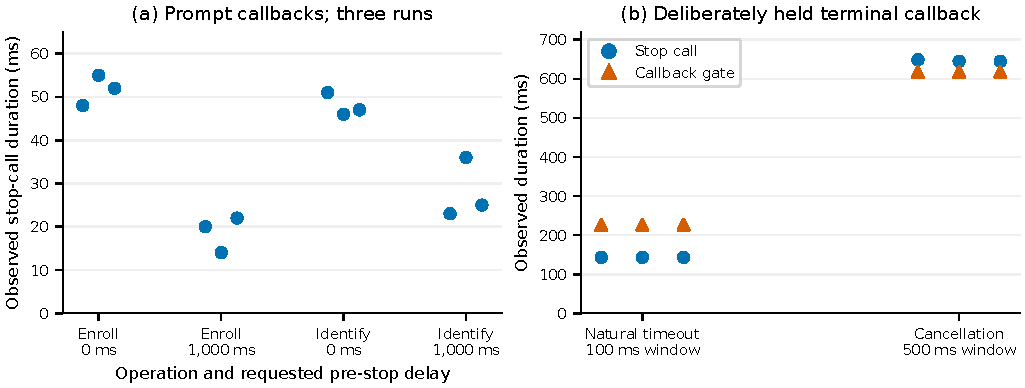
\includegraphics[width=\textwidth]{figures/fig_eval_lifecycle.pdf}
\caption{AI10 stop behavior. (a) Three observations per primary cancellation case with promptly returning callbacks; zero delay means no added sleep before stop. (b) Separate held-callback tests with 100 or 500~ms added observation windows. Gate duration includes probes and logging; these stress timings must not be pooled with ordinary cancellation latency.}
\label{fig:eval_lifecycle}
\end{figure*}

A second suite held the terminal callback on a semaphore during natural enrollment timeout and continuous-identification cancellation. Three repetitions per case produced six held callbacks and six subsequent recovery operations. All 24 enrollment, identification, callback-replacement, and inventory probes returned \texttt{-EBUSY}. Natural-timeout probes preceded the first stop call, excluding a stopping caller's mutex as the sole explanation. A second stop caller was rejected in all six cases.

The primary stop remained pending through the added observation window. After gate release, the marker immediately before callback return preceded the marker after stop return, and recovery succeeded. Natural-timeout stop calls took 143~ms; cancellation stop calls took 645--649~ms (Figure~\ref{fig:eval_lifecycle}(b)). The exact callback-return instruction was not instrumented, and millisecond timestamp equality does not imply zero delay.

Across both suites, all 54 accepted operations produced one terminal event. The observed exclusion, pending-stop behavior, and marker ordering support the specified obligations for the tested schedules and demonstrate the effect of callback duration on availability.

\subsection{E3: Scheduling Responsiveness}
\label{sec:eval_scheduling}

A periodic task performed fixed integer work calibrated to approximately 200~$\mu$s, with a 10~ms period and relative deadline. Its priority was 2 or 8; lower values take precedence. Biometric work used priority~5. Optional background work at priority~4 executed a calibrated 3,513~$\mu$s every 7~ms, representing 50.19\% offered computation rather than measured CPU utilization.

Each device ran initialized-idle and repeated synchronous identification conditions, the latter with a separate caller and one-second timeout. AI10 additionally ran asynchronous single-attempt identification, waiting for termination and callback quiescence before restarting; its coordinator and worker both used priority~5. Synchronous callers suspended normally without scheduler locking or artificial busy-waiting.

After a 200~ms settling interval, each condition recorded 300 periodic jobs over approximately three seconds. Active conditions required a completed biometric cycle within the window; in-flight work was drained afterward. Records were buffered and printed after measurement.

For timer-callback release $r_i$, task start $s_i$, finish $f_i$, and cycle frequency $f_c$, the recorded quantities were
\begin{equation}
D_i=\frac{s_i-r_i}{f_c},\quad
R_i=\frac{f_i-r_i}{f_c},\quad
W_i=\frac{f_i-s_i}{f_c}.
\label{eq:eval_timing}
\end{equation}
Here $D_i$ is release-to-start latency, $R_i$ response time, and $W_i$ execution span including preemption. A miss means $R_i>10$~ms. This definition excludes lateness before the timer-callback timestamp and does not measure response against an ideal external schedule.

Three suites per device, with 12 AI10 or eight fingerprint conditions per suite, produced 25,200 jobs across 84 measurement cells. Suites are repetitions; jobs within a suite are correlated observations. Mode order varied, while device and priority/load group orders remained fixed. Checks covered receive status, job counts, queue loss, timestamp ordering and wrap, and workload progress. Percentiles use linear interpolation within each 300-job cell, retaining the three suite results separately.

\begin{figure*}[t]
\centering
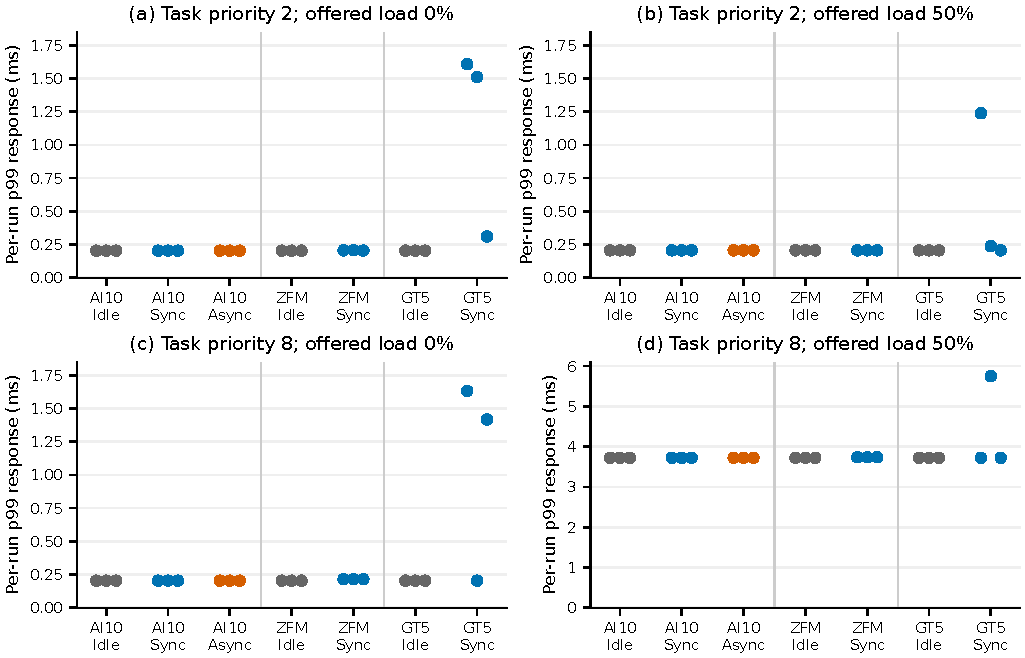
\includegraphics[width=\textwidth]{figures/fig_eval_p99.pdf}
\caption{Per-run 99th-percentile response times: 84 points, each summarizing 300 jobs, with three points per condition. Priority~2 places the task above the workload threads; priority~8 places it below them. Panel~(d) uses a different vertical scale. Asynchronous operation is tested only on AI10.}
\label{fig:eval_p99}
\end{figure*}

All suites passed completeness and progress checks without queue loss, receive errors, or observed deadline misses. Figure~\ref{fig:eval_p99} summarizes per-run 99th-percentile response times. AI10's priority-2 maxima did not exceed 0.213~ms. ZFM-X0 synchronous maxima approached 0.641~ms despite 99th percentiles near idle. GT-5X showed greater variation: its unloaded priority-2 synchronous 99th percentiles were 1.608, 1.511, and 0.311~ms (Figure~\ref{fig:eval_p99}).

At priority~8 with background load, idle maxima were approximately 3.722~ms. Active maxima were 3.764/3.765~ms for synchronous/asynchronous AI10, 4.163~ms for ZFM-X0, and 6.333~ms for GT-5X. GT-5X's loaded synchronous 99th percentiles ranged from approximately 3.722 to 5.747~ms. Figure~\ref{fig:eval_ecdf} retains individual-run distributions rather than pooling their differing tails.

\begin{figure*}[!h]
\centering
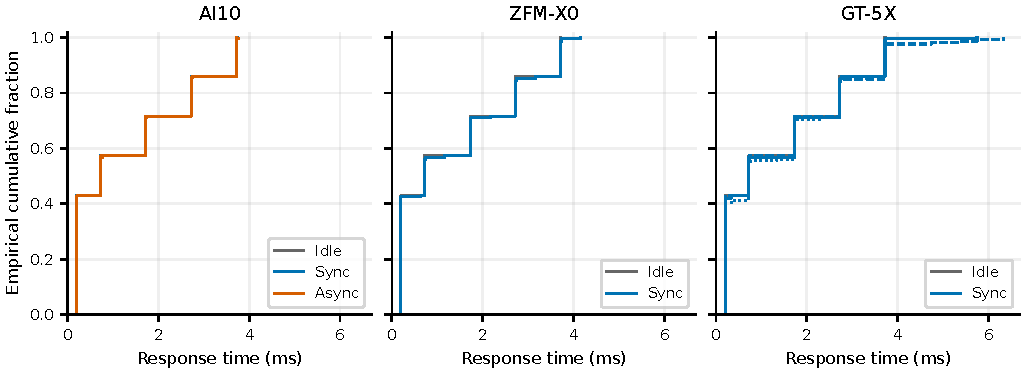
\includegraphics[width=\textwidth]{figures/fig_eval_ecdf.pdf}
\caption{Response-time distributions at priority~8 with nominal 50\% offered background computation. Each curve contains 300 jobs; the subset contains 21 curves and 6,300 jobs. Line styles distinguish the three runs. Curves may overlap.}
\label{fig:eval_ecdf}
\end{figure*}

The measurements capture combined effects of UART rates, traffic, synchronization, and module responses; they do not isolate the cause of GT-5X's spikes. AI10's synchronous and asynchronous interference was similar under the no-sample workload, consistent with synchronous callers suspending while unrelated work proceeds. Observed maxima are not worst-case bounds.

\subsection{E4: Resource Footprint}
\label{sec:eval_resources}

Each driver had biometrics-disabled UART/console, initialized-idle, and synchronous-identification builds; AI10 also had an asynchronous build. All used size optimization, a 4,096-byte main stack, disabled shell/logging, and no stack-fill profiling. Separate instrumented builds enabled stack initialization and an observer.

Table~\ref{tab:eval_memory} reports increments from Zephyr's native linked ROM/RAM reports. Every matched baseline contained 57,600 bytes ROM and 126,204 bytes RAM. Increments include application code, dependencies, and alignment; ESP32 executable RAM and shared platform storage require linker-map interpretation.

\begin{table}[t]
\centering
\caption{Linked-image increments over matched baselines, in bytes. Instrumented stack-profile builds are excluded.}
\label{tab:eval_memory}
\small
\renewcommand{\arraystretch}{1.1}
\setlength{\tabcolsep}{5pt}
\begin{tabular}{|l|l|r|r|}
\hline
\textbf{Driver} & \textbf{Mode} &
$\Delta$\textbf{ROM} & $\Delta$\textbf{RAM} \\ \hline
ZFM-X0 & Idle  & 4,924 & 648 \\ \hline
ZFM-X0 & Sync  & 4,972 & 648 \\ \hline
GT-5X  & Idle  & 5,172 & 152 \\ \hline
GT-5X  & Sync  & 5,220 & 152 \\ \hline
AI10   & Idle  & 5,280 & 3,824 \\ \hline
AI10   & Sync  & 5,328 & 3,824 \\ \hline
AI10   & Async & 5,712 & 3,840 \\ \hline
\end{tabular}
\end{table}

Synchronous integration added 4,972--5,328 bytes ROM. AI10 reserves its 2,048-byte worker stack, 1,024-byte receive ring, packet storage, and synchronization state even in idle and synchronous builds. Its asynchronous application therefore adds only 384 bytes ROM and 16 bytes RAM over the synchronous image.

GT-5X's 152-byte instance contains a pointer to heap storage. Source inspection identifies simultaneous initialization requests for a persistent 498-byte template buffer and a temporary 30-byte packet: 528 payload bytes, excluding allocator overhead and fragmentation. Template transfers would request another 504-byte packet but were not profiled. These are requested sizes, not measured peak heap use. Heap backing storage is already included in linked RAM; adding these payloads to image totals would double-count it, while the instance size alone omits runtime demand.

At quiescent checkpoints, an observer scanned the blocked application stack and AI10 worker. Each device completed three no-sample synchronous attempts; AI10 additionally completed three asynchronous timeouts and three continuous-recognition cancellations. Maximum observed main-stack watermarks were 576, 592, and 688 bytes for ZFM-X0, GT-5X, and AI10, respectively, from 4,096-byte stacks. AI10's worker watermark was 528 bytes from 2,048 bytes.

Watermarks include startup and harness work, and the worker measurement includes the test callback. They characterize the exercised workloads, not worst-case stack requirements; an unchanged watermark does not imply zero stack use.

\subsection{Research Question Answers and Limitations}
\label{sec:eval_limits}

For RQ1, one application source reused coordination across three device families through capability-dependent workflows while retaining explicit allocation, termination, and recovery policies. For RQ2, all 54 accepted operations delivered one terminal event, and directed checks supported exclusion and callback quiescence for the tested schedules. For RQ3, interference varied with driver, priority, and load; AI10's synchronous and asynchronous paths behaved similarly under the no-sample workload. For RQ4, linked-image costs and observed stack usage exposed implementation-dependent allocation choices, including worker storage retained during synchronous use. Together, these findings support reusable coordination while requiring configuration-specific timing and memory assessment.

Coverage is limited to one board, one specimen per family, and one operator. Functional runs establish workflow behavior, not recognition accuracy or calibrated security equivalence. Shared recovery tests cover staged abort after one capture and AI10 cancellation without a sample; they do not establish recovery after uncertain storage.

Asynchronous lifecycle evidence is limited to AI10 and the directed schedules. Delayed stops across ownership handoff, completion/cancellation races, cleanup failure after acknowledged storage, and systematic UART fault injection were not evaluated. Scheduling evidence covers short, no-sample workloads with three suites per device and fixed device and priority/load group orders.

\section{Conclusion}
\label{sec:conclusion}

BASE provides a unified biometric driver class combining capability discovery, typed operations and results, and explicit lifecycle rules. Its Zephyr implementation supports shared application workflows across staged fingerprint and device-managed face/palm modules while preserving distinctions between enrollment control, device persistence, and host-side operation lifetime.

One application reused coordination logic across three
device families. Directed AI10 tests supported the specified
termination, exclusion, and quiescence obligations for the
exercised schedules. Scheduling and resource measurements
showed that integration costs depend on driver execution
and allocation choices, including callback duration and
worker storage retained during synchronous use.

The resulting abstraction supports shared workflows while
keeping device-specific effects and application ownership
responsibilities explicit. Further work should examine
completion/cancellation races, uncertain-storage recovery,
successful-acquisition workloads, and transfer to other RTOSs.
\section*{Acknowledgment}
The authors thank the Zephyr Project Architecture Working Group for its technical review and feedback on the biometrics subsystem architecture. We also thank the SUST research center for funding the experimental equipment.


% To print the credit authorship contribution details
\printcredits

%% Loading bibliography style file
% \bibliographystyle{model1-num-names}
\bibliographystyle{elsarticle-num-names}

% Loading bibliography database
\bibliography{cas-refs}

% Biography
\bio{}
Md~Siratul~Islam is pursuing the B.Sc. degree in Physics at Shahjalal University of Science and Technology (SUST), Sylhet, Bangladesh. He serves as a Research Assistant in the Department of Electrical and Electronic Engineering at SUST.

He authored and maintains the FIDO2 and biometrics subsystems in Zephyr RTOS. He also maintains some Linux kernel drivers and reviews patches in the Linux Industrial I/O (IIO) subsystem. His research interests include embedded systems, real-time operating systems, device-driver architecture, and secure authentication on resource-constrained devices.
\endbio

\bio{}
Md~Rasedujjaman is currently with the Department of Electrical and Electronic Engineering, Shahjalal University of Science and Technology (SUST), Sylhet, Bangladesh. His research interests include optical systems, signal processing, and IoT security protocols.
\endbio

\end{document}
